
\begin{exercice}[Pirates et équidistance]
Les pirates Olivier Levasseur et Anne Bonny se disputent un diamant. Jo l'intello cherche une méthode équitable pour savoir qui aura la pierre précieuse. Reproduis précisément les parchemins que dessine Jo, au fur et à mesure de la discussion.
\begin{enumerate}
 \item « Vous n'avez qu'à vous placer à 50 pas l'un de l'autre, et mettre le diamant au milieu ». 
 
Il fait un premier dessin sur un parchemin pour schématiser sa proposition, en représentant 10 pas par 1 centimètre.
 \item Les pirates estimant que la course n'est pas assez longue pour les départager, Jo propose un second schéma : « Vous vous mettez toujours à 50 pas l'un de l'autre, mais vous mettez le diamant à 70 pas de chacun de vous. Je me placerai au milieu de vous deux. ». \\[-0.9em]
 \item Jo réfléchit, puis propose un troisième schéma : « On n'a qu'à se mettre tous les trois à 70 pas du diamant et vous vous placerez à 100 pas de moi ».
 \end{enumerate}
\end{exercice} 


\begin{exercice}[À partir d'une figure (bis)]
On considère la figure suivante :
\begin{center} 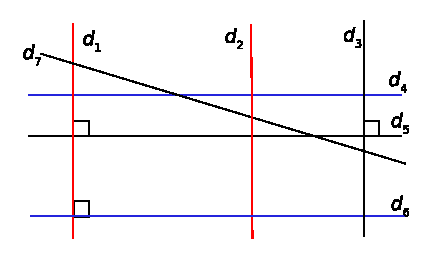
\includegraphics[width=5.8cm]{droites-sec-paral} \end{center}
On donne de plus : $d_1 \parallel d_2$ et $d_4 \parallel d_6$.
 \begin{enumerate}
  \item Reproduis cette figure et ajoute tous les angles droits possibles.
  \item Quelles sont les droites parallèles à $d_3$ ?
  \item Quelles sont les droites parallèles à $d_6$ ?
  \item Quelles sont les droites sécantes à $d_7$ ?
  \end{enumerate}
\end{exercice}


\begin{exercice}[Partage équitable]
Marie organise une soirée avec cinq de ses amis. Ils achètent une pizza et une tarte, toutes deux de forme circulaire.
\begin{enumerate}
 \item Comment doit procéder Marie pour partager équitablement sa pizza avec ses amis ?
 \item Au moment du dessert, ses parents, son frère et sa sœur se joignent à la petite fête. Marie doit découper la tarte équitablement. Comment procède‑t‑elle ?
 \end{enumerate}
\end{exercice}


\begin{exercice}[Des histoires de milieux]
Construis $d_1$ et $d_2$ deux droites perpendiculaires en $O$. $A$ est un point de $d_1$ et $B$ un point de $d_2$. $C$ est le point de $d_1$ tel que $O$ soit le milieu de $[AC]$ et $D$ le point de $d_2$ tel que $O$ soit le milieu de $[BD]$.
\begin{enumerate}
 \item Que représente $d_1$ pour $[BD]$ ? Et $d_2$ pour $[AC]$ ? Justifie tes réponses.
 \item Place $I$ le milieu de $[AB]$ et $I'$ le point de $(OI)$ tel que $O$ soit le milieu de $[II']$.
 \item Où semble être placé le point $I'$ ?
 \item Comment semblent être les droites $(AD)$, $(II')$ et $(BC)$ ?
 \end{enumerate}
\end{exercice}


\begin{exercice}
Voici le croquis d'un pilier réalisé par un architecte :
\begin{center} 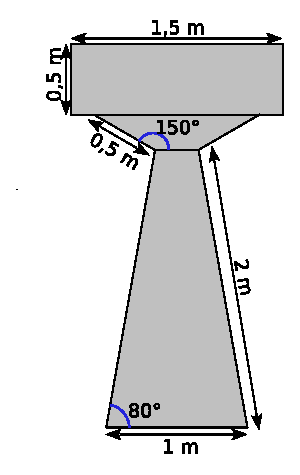
\includegraphics[width=3.9cm]{pilier} \end{center}
Construis ce pilier à l’échelle suivante : 3 cm sur la figure représentent 1 m dans la réalité.
\end{exercice}

%%%%%%%%%%%%%%%%%%Mise en page
\newpage
%%%%%%%%%%%%%%%%%%%%%%%%%%%%%%

\begin{exercice}[Orion]
Alex observe la constellation d'Orion dans le ciel au travers de son télescope. Il voudrait la représenter pour son prochain exposé. Pour cela, il réalise quelques mesures ; il a reporté ses observations sur le croquis ci‑dessous.

Construis pour Alex la constellation d'Orion.
\begin{center} 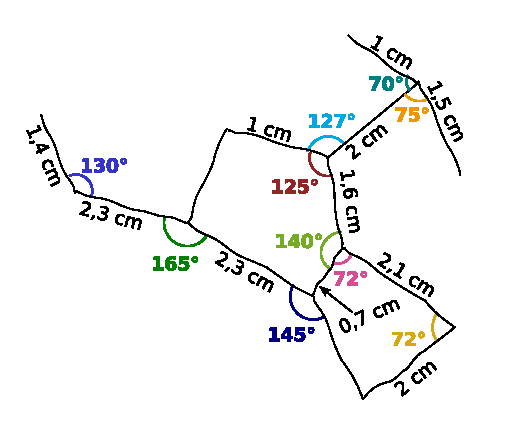
\includegraphics[width=7.1cm]{orion1} \end{center}
\begin{center} $\boxed{
\includegraphics[width=4cm]{orion2}}$ 

{\footnotesize\emph{La constellation d'Orion.}} \end{center}
\end{exercice}
